\documentclass[11pt,a4paper]{article}
\pagestyle{myheadings}

\usepackage[pdftex]{graphicx}
\usepackage{listingsutf8}
\usepackage{hyperref}

\usepackage{amsmath}
\usepackage{verbatim}
\usepackage{moreverb}

\usepackage[utf8]{inputenc}    % use utf-8 encoding
\usepackage[ngerman]{babel}    % use german date format
\usepackage[T1]{fontenc} 
\lstset{language=Java,tabsize=2,numbers=left,numberstyle=\tiny,breaklines=true,basicstyle=\fontsize{8}{10}\selectfont}

\author{Thomas Fischl (s1310454009@students.fh-hagenberg.at)}
\newcommand{\num}{1}
\newcommand{\subject}{SVE}
\renewcommand{\figurename}{Abbildung}
\markright{\subject, Studentenprojekt, Thomas Fischl (s1310454009@students.fh-hagenberg.at)}

\newcommand{\changefont}[3]{\fontfamily{#1} \fontseries{#2} \fontshape{#3} \selectfont}

\makeatletter
\newcommand\textsubscript[1]{\@textsubscript{\selectfont#1}}
\def\@textsubscript#1{{\m@th\ensuremath{_{\mbox{\fontsize\sf@size\z@#1}}}}}
\newcommand\textbothscript[2]{%
  \@textbothscript{\selectfont#1}{\selectfont#2}}
\def\@textbothscript#1#2{%
  {\m@th\ensuremath{%
    ^{\mbox{\fontsize\sf@size\z@#1}}%
    _{\mbox{\fontsize\sf@size\z@#2}}}}}
\def\@super{^}\def\@sub{_}

\catcode`^\active\catcode`_\active
\def\@super@sub#1_#2{\textbothscript{#1}{#2}}
\def\@sub@super#1^#2{\textbothscript{#2}{#1}}
\def\@@super#1{\@ifnextchar_{\@super@sub{#1}}{\textsuperscript{#1}}}
\def\@@sub#1{\@ifnextchar^{\@sub@super{#1}}{\textsubscript{#1}}}
\def^{\let\@next\relax\ifmmode\@super\else\let\@next\@@super\fi\@next}
\def_{\let\@next\relax\ifmmode\@sub\else\let\@next\@@sub\fi\@next}

\makeatother

\begin{document}

\title{Sensordatenverarbeitung auf Basis von AKKA und Tomcat}
\maketitle

\section{Ziel}

Im Zeitalter von IoT (Internet of Things) ist es essentiell, große Datenmengen an Sensordaten zu verwalten. Dazu gehört auf der einen Seite, dass man die Sensordaten von vielen unterschiedlichen Devices über das Internet oder einem anderem Netzwerke empfangen kann. Dabei muss der Server mit einer großen Anzahl von parallelen Verbindungen umgehen können. Auf der anderen Seite muss die empfangene Nachricht so schnell wie möglich gespeichert und verarbeitet werden. In diesem Szenario ist der Verlust von ein paar Nachrichten nicht so schlimm. Es wird ein größeres Augenmerk auf die vertikale Skalierung und Ausfallsicherheit gelegt.

\section{Das AKKA Framework}

Das AKKA Framework (\href{http://akka.io}{akka.io}) ist eine Implementierung des Aktor-Model (\href{http://en.wikipedia.org/wiki/Actor_model}{Link}).
Bei diesem Ansatz, wird die Anwendungslogik mit hilfe von Aktoren implementiert.

Dabei werden jedoch die Aufrufe zwischen einzelnen Aktoren nicht über Methoden- oder Funktionsaufrufe umgesetzt. Aktoren können nur über Messages miteinander kommunizieren. Das Konzept ist aber nicht mit dem Nachrichten austausch aus OOP vergleichbar, wo ein Objekt einem anderem Objekt eine Nachricht schicken kann. Diese Konzept lässt sich viel besser mit ein JMS-System, ESB (Enterprise Service Bus) oder SOA vergleichen. Der Unterschied zu den vorher genannten System liegt darin, dass diese prozess- bzw. systemübergreifend agieren und AKKA in einem Prozess läuft (solange man keinen AKKA Cluster betreibt). Dadurch schafft man, dass die Aktoren sehr lose miteinander gekoppelt sind. Diese Eigenschaft verleiht einem Aktorensystem gute Skalierungseigenschaft.
\\
Aus der AKKA Community (bzw. Scala) ist auch eine neue Bewegung heraus entstanden die ein Manifest (http://www.reactivemanifesto.org/) verfasst haben. In diesem Manifest werden die Eigenschaften und Grundzüge von reaktiven Anwendungen beschrieben. Die Haupteigenschaften einer reaktiven Anwendung sind
'Responsive', 'Scalable', 'Resilient' und 'Event-Driven'. Diese Basis für diese Art von Anwendungen kann das AKKA Framework sein.


\section{Lösungsidee}


Das Ziel dieses Projektes ist es, eine reaktive Anwendung auf Basis von AKKA zu entwickeln. Diese Anwendungen soll sehr gut Skalierungseigenschaften aufweisen. Wünschenswert wäre ein System, welches möglichst automatisch vertikal skalieren kann. \\
\\
Um einen Vergleich für die Messergebnisse zu erhalten, wird parallel noch eine zweite Anwendungen implementiert, welche auf die klassischen Methoden aufsetzt. Für die beiden Anwendung soll die gleiche Anwendungslogik verwendet werden. Der Unterschied der Anwendungen soll lediglich in der Art und Weise der Resourceverwaltung liegen. Dabei sollen die Resourcen (CPU und RAM) von modernen System möglichst gut ausgenutzt werden. Dabei sprechen wir von Multicore-Servern mit bis zu 64 oder 128 Cores und bis zu mehreren 100 GBs von RAM. Jedoch soll die Anwendung nicht explizit für diese großen Multicore-Server entwickelt werden. Die Anwendung soll im besten Fall mit den vorhanden Resourcen von einem Server mitwachsen können.\\

\begin{figure}[h]
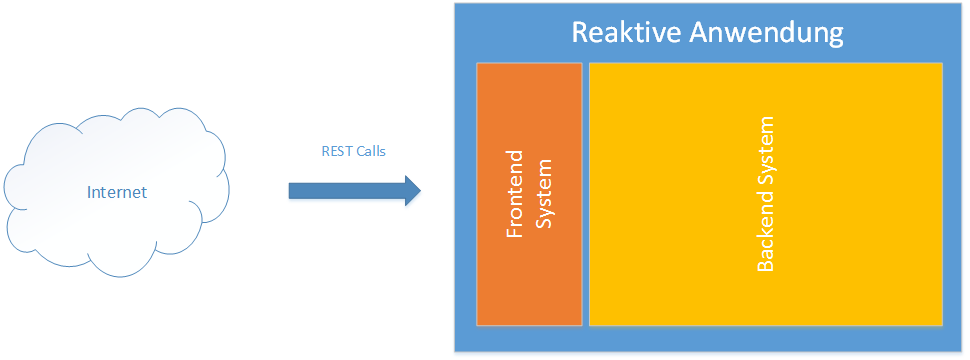
\includegraphics[width=1\textwidth]{../pic/architektur.png}
\label{fig:test}
\end{figure}

Die Anwendung wird aus zwei Teilen bestehen. Der erste Teil ist für die Annahme von HTTP Request zuständig. Damit soll es möglich sein, dass man die Sensordaten im JSON Format an den Server schicken kann. Die besondere Aufgaben von diesem Teil der Anwendung ist es, dass eine große Anzahl an Anfragen parallel abgearbeitet werden müssen.\\
\\
Der zweite Teil der Anwendung ist für die Abarbeitung der Sensordaten zuständig. Für diese Beispiel beschränkt sich der Funktionsumfang auf das Schreiben der Daten und das pseudomäßige verarbeiten der Daten. Hier ist es sehr wichtig, dass die Arbeit möglichst gut auf alle verfügbaren Resourcen aufteilen werden kann.

\section{Umsetzung}

Auf Basis der Überlegungen aus dem vorgehenden Kapiteln wird die Anwendung mit den beiden Frameworks Tomcat(http://tomcat.apache.org/) und AKKA umgesetzt. \\
\\
Tomcat wird für das Frontend der Anwendung verwendet. Die Anwendung startet den Tomcat-Server im Embeeded Modus. D.h. der Tomcat-Server läuft nicht in einem eigenen Prozess, sondern wird in einer bestehenden JVM gehostet. Für die Anwendungslogik werden Servlets implementiert. Diese Servlets verarbeiten die REST Anfrage und leiten diese an das Backend weiter. Die Anwendung besteht aus zwei Servlets. Das eine Servlet verarbeitet die REST Anfrage synchron und die zweite asynchron.\\
\\
Das AKKA Framework wird für die Backend-Implementierung verwendet. Dabei wird die Verarbeitung im AKKA System über ein Nachricht aus dem Servlet angestoßen. Das AKKA System ist dabei aus zwei Aktoren aufgebaut. Der FrontendAktor ist für die Verteilung der REST Anfragen verantworlich und retuniert das Ergebnis. Der SensorDataStoreWorker ist für die tatsächliche Abarbeitung der Anfragen verantwortlich. In diesem Schritt, wird die Anfragen schon in zwei Nachrichten aufgeteil. Die Nachricht SensorDataStoreMsg veranlasst den Aktor dazu, die Sensordaten zu speichern. Diese Nachricht wird vom Aktor mit keiner weitern Nachricht bestätigt, also ein klassischen 'Fire and Forget'. Die zweite Nachricht löst das Verarbeiten der Sensordaten aus. Auf diese Nachricht schickt der Worker Aktor eine Antwort mit dem Ergebnis zum Sender zurück. \\

Im weitern werden die drei unterschiedlichen Ausbaustufen der Anwendung beschrieben.

\subsection{Ausbaustufe 1: Klassische synchrone Implementierung}

In der ersten Implementierung werden die Sensordaten synchron im Servlet-Thread abgearbeitet und das AKKA Framework kommt nicht zum Einsatz. D.h. für die Zeit der Abarbeitung wird ein Tomcat-Worker-Thread blockiert. Das resultiert in einem Thread-Engpass bei den Tomcat-Worker-Threads und der Server kann keine neuen Verbindungen annehmen. Das Ergebnis ist, dass der Server nicht mehr auf neue Anfragen reagiert und instabil wird.\\
\\
Dieses Problem versucht die zweite Ausbaustufe der Anwendung zu lösen.

\subsection{Ausbaustufe 2: Asynchrone Verarbeitung}

Bei der asynchrone Verarbeitung wird ein Servlet Container benötigt, welcher den JSR 315 - Servlet 3.0 implementiert. Mit diesem JSR ist es möglich, die Abarbeitung der HTTP Anfragen asynchron auszuführen. In dieser Anwendung wird ein Tomcat Server in der Version 8.0.8 verwendet. Die grundlegende Änderung ist im Servlet. Dort wird in der doGet Methode ein asynchroner Kontext gestaret und danach wird gleich der Tomcat-Worker-Thread wieder frei gegeben. Dadurch kann der Server mehr Request gleichzeitig servisieren. Im asynchronen Kontext wird das AKKA System angestoßen, indem die initiale Nachricht 'SensorDataWorkMsg' in das System geschickt wird. Diese Nachricht wird vom 'AkkaFrontendMaster' Aktor verarbeitet. Dabei wird die initiale Nachricht in zwei Unternachrichten aufgeteilt. Die eine ist für das Speichern der Daten zuständig und die zweite ist für das Verarbeiten der Daten und das Berechnen des Resultates verantwortlich. Diese beiden Nachrichten werden von dem 'AkkaSensorDataStoreWorker' Aktor verarbeitet. Das Ergebnis wird mit der Nachricht 'SensorDataWorResultMsg' zurück gesendet und mit der Abarbeitung der Servlet-Anfrage fortgefahren.\\
\\
Diese Ausbaustufe hat nun das Problem der vielen parallen Anfragen gelöst. Jedoch wurde noch nicht das Problem der optimalen Resourcenauslastung gelöst. Diese Problem wird in der letzten Ausbaustufe behandelt.

\begin{figure}[h]
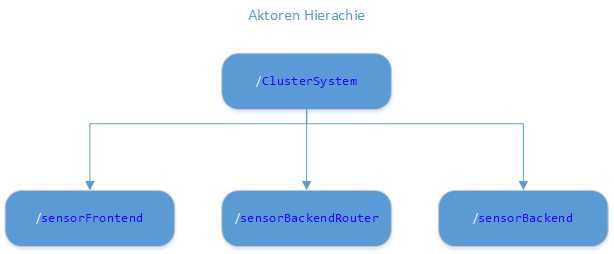
\includegraphics[width=1\textwidth]{../pic/aktorsystem.png}
\label{fig:test}
\end{figure}

\subsection{Ausbaustufe 3: AKKA Cluster}

In dieser Ausbaustufe wird die bisherige Anwendung in mehrere Prozesse aufgeteilt, ohne Änderungen an der Anwendungslogik vornehmen zu müssen. \\
\\
Um die Anwendungslogik auf mehrere Prozesse aufteilen zu können wird das bestehende AKKA System umkonfiguriert. Es wird ein AKKA Cluster konfiguriert, welcher aus einem Frontend und einem Backend Teil besteht. Der Frontend Teil des Clusters wird mit dem Tomcat-Server mit gestartet. Dieser Frontend Teil enthält nur den 'AkkaFrontendMaster' Aktor. Der zweite Aktor, welcher für die Abarbeitung zuständig ist, wird in diesem Prozess nicht gestartet. Dafür können beliebt viele Backend-AKKA-Prozesse gestartet werden. Diese Backend-Prozesse melden sich am Cluster an. Der Cluster verteilt dann die Nachrichten gleichmäßig auf alle Backend-Prozesse. Mit diesem einfachen System hat man ein dynamisch vertikal skalierbares System geschaffen, welches alle beschriebenen Anforderungen erfüllt. 

\section{Essentielle Source-Code Ausschnitte}

\subsection{AkkaFrontendMaster.java}
\begin{lstlisting}
public class AkkaFrontendMaster extends UntypedActor {

  ...
  
  // Define the loadbalancing capability for the workers
  protected void init() {
    workerRouter = this.getContext().actorOf(Props.create(AkkaSensorDataStoreWorker.class).withRouter(new RoundRobinPool(nrOfWorkers)), "workerRouter");
  }

  // Handle incoming messages
  @Override
  public void onReceive(Object msg) throws Exception {
    if (msg instanceof SensorDataWorkMsg) {
      workerRouter.tell(new SensorDataStoreMsg((SensorDataWorkMsg) msg), getSelf());
      workerRouter.tell(new SensorDataProcessMsg((SensorDataWorkMsg) msg), getSelf());
    } else if (msg instanceof SensorDataWorResultMsg) {
      SensorDataWorResultMsg msgObj = (SensorDataWorResultMsg) msg;
      facade.finishRequest(msgObj.getSessionId(), msgObj.getGroup());
    }
  }
}
\end{lstlisting}

\subsection{AkkaSensorDataStoreWorker.java}
\begin{lstlisting}
public class AkkaSensorDataStoreWorker extends UntypedActor {

  @Override
  public void onReceive(final Object msg) throws Exception {
    if (msg instanceof SensorDataStoreMsg) {
      // Store sensor data
      ...
    } else if (msg instanceof SensorDataProcessMsg) {
      // Process the sensor data and return the result
      ...
      actorSender.tell(new SensorDataWorResultMsg(msgObj.getMessage().getSessionId(), result), actorSelf);
    }
  }
}
\end{lstlisting}

\subsection{Cluster.conf}
\begin{lstlisting}
akka {
  remote {
    log-remote-lifecycle-events = off
    netty.tcp {
      hostname = "127.0.0.1"
      port = 0
    }
  }
  cluster {
    seed-nodes = [
      "akka.tcp://ClusterSystem@127.0.0.1:2551",
      "akka.tcp://ClusterSystem@127.0.0.1:2552",
      "akka.tcp://ClusterSystem@127.0.0.1:2553",
      "akka.tcp://ClusterSystem@127.0.0.1:2554"
    ]
    auto-down-unreachable-after = 10s
  }
}

akka.actor.deployment {
  /sensorFrontend/sensorBackendRouter = {
    router = adaptive-group
    metrics-selector = mix
    nr-of-instances = 100
    routees.paths = ["/user/sensorBackend"]
    cluster {
      enabled = on
      use-role = backend
      allow-local-routees = off
    }
  }
}
\end{lstlisting}

\subsection{AsyncRestSensorServlet.java}
\begin{lstlisting}
@WebServlet(name = "AsyncRestSensorServlet", urlPatterns = { "/async/rest/*" }, asyncSupported = true)
public class AsyncRestSensorServlet extends HttpServlet {

  private AkkaFrontendFacade frontend = new AkkaFrontendFacade();

  protected void doGet(HttpServletRequest req, HttpServletResponse resp) throws ServletException, IOException {
    final AsyncContext asyncCtx = req.startAsync();
    asyncCtx.start(new AsyncHttpRequestHandler(asyncCtx));
  }

  private final class AsyncHttpRequestHandler implements Runnable {
    public void run() {
      HttpServletRequest req = (HttpServletRequest) asyncCtx.getRequest();
      HttpServletResponse resp = (HttpServletResponse) asyncCtx.getResponse();

      try {
        processRequest(req, resp);
      } catch (IOException e) {
        errorCounter.mark();
        e.printStackTrace();
        throw new RuntimeException(e);
      }
    }

    private void processRequest(HttpServletRequest req, final HttpServletResponse resp) throws IOException {
      ...
      
      // Send the inital akka message
      frontend.processSensorData(userId, group, new ResponseHandler() {
        public void process(SensorDataGroup result) {
          try {
            // Write result on response stream
          } finally {
            asyncCtx.complete();
          }
        }
      });
    }
  }
}
\end{lstlisting}


\section{Resultate}

Um die Überlegungen aus den vorgehenden Kapiteln zu verifizieren wurden Lasttests gegen die drei Implementierungen ausgeführt.\\
\\
Für die Lasttests wurde Borland Silk Performer verwendet. Der Lasttest simuliert 1000 parallelen Clients. Diese virtuellen Clients werden mit jeweils einer eigenen Verzögerung gestartet. Nach 5 Minuten sind alle 1000 Clients gestaret. Der Lasttest läuft insgesamt 10 Minuten. Daraus ergibt sich, dass der Server jeweils 5 Minute unter voller Last steht. Als Performance Vergleich zwischen den drei Ausbaustufen wurde die 'HTTP Response Time' verwendet. \\
\\
Die gesamten Lasttests wurden auf einem Computer mit einer i7-4790 CPU mit 3.6 GHz und 8 Cores und mit 16 GB Ram durchgeführt.

\subsection{HTTP Response Time - Grafik}

Die Grafik zeigt, dass es keine großen Unterschied bei der 'Response Time' zwischen der Ausbaustufe 1(blau) und 2(grün) gibt. Das Erklärt sich einfach daraus, dass beide dieselbe Anzahl an Worker Threads zur Verfügung hatten. Die dritte Line (rot) zeigt, dass die dritte Ausbaustufe wunderbar vertikal skaliert. Die ersten 5 Minuten das Lasttests wurde der Cluster mit 2 Nodes betrieben. Nach 5 Minuten, wenn die volle Last am System vorhanden ist, wurden zwei weiter Cluster Nodes gestartet. Man nach ca. 15 Sekunden sehen, dass die 'Response Time' deutlich zurück geht. 

\begin{figure}[h]
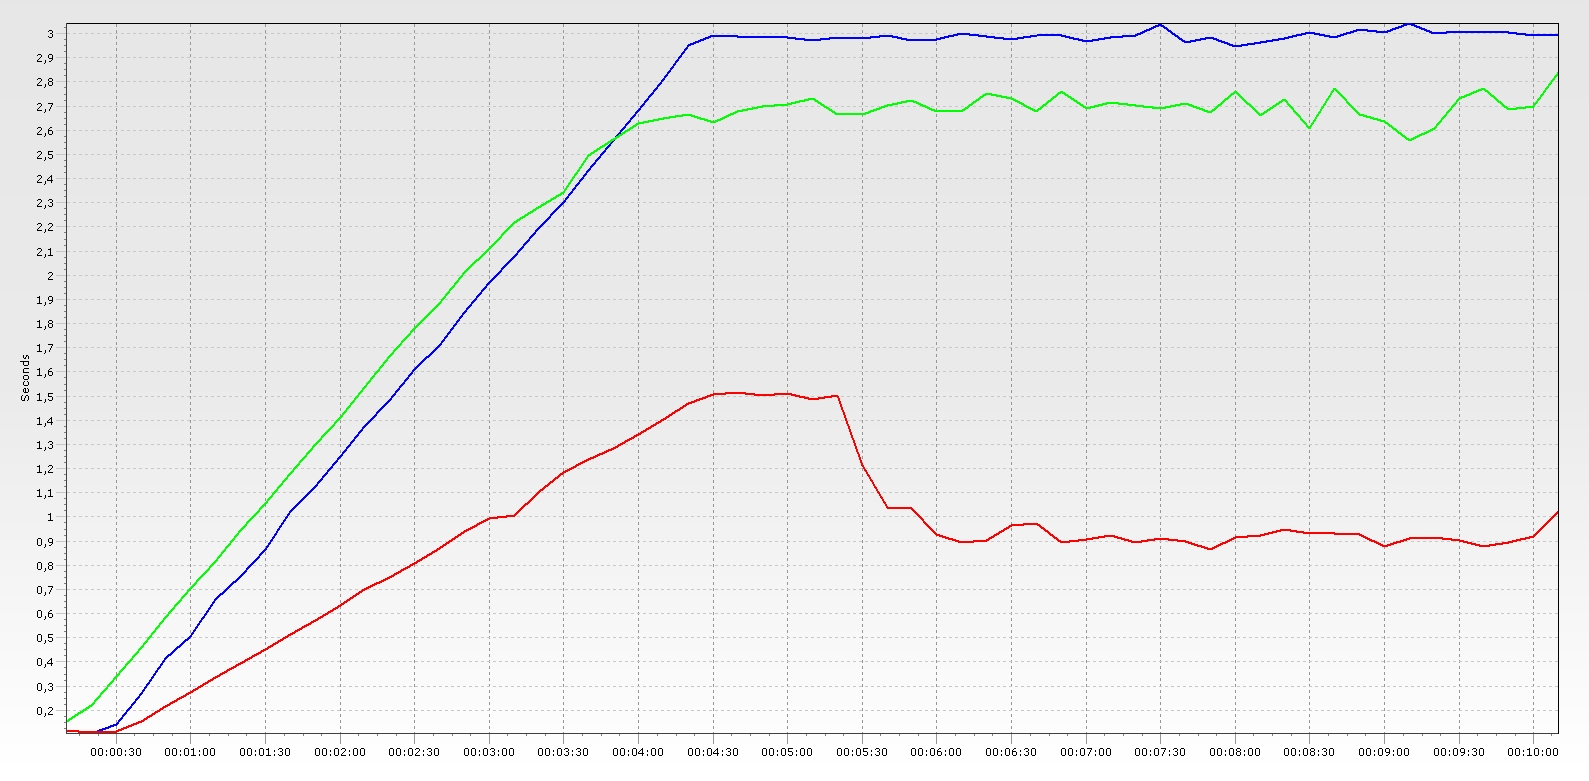
\includegraphics[width=1\textwidth]{../pic/Response-time.jpg}
\label{fig:test}
\end{figure}

\pagebreak
\subsection{Load Test Overview Report}

In den nächsten Unterkapiteln sieht man einen Overview Report für jede Ausbaustufe mit den vier wichtigsten Kennzahlen: Active Users (Lila), Average Number of Transactions per Second (Grün), Number of HTTP Errors (Rot) und Transaction Response Times (Blau). 

\subsubsection{Overview Report - Ausbaustufe 1}

Bei der ersten Ausbaustufe kann man ganz klar sehen, dass bei ca. 500 parallelen Devices der Server instabil wird. Zu dieser Zeit steigt die Zahl der HTTP Fehler an. Die Ursache für diese Fehler ist, dass der Server keine weiteren Verbindungen mehr servisieren kann. 

\begin{figure}[h]
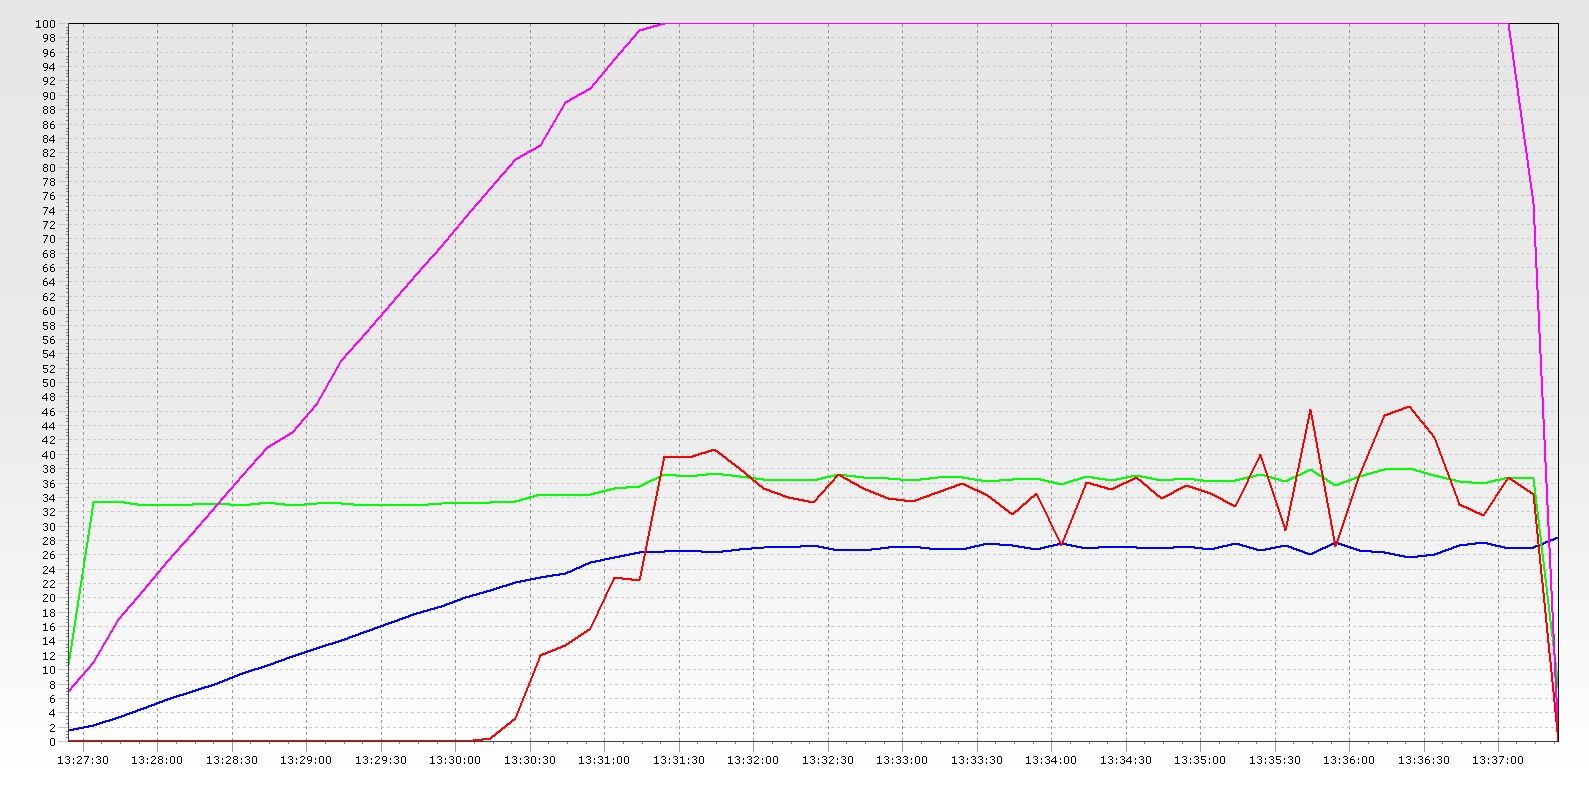
\includegraphics[width=0.9\textwidth]{../pic/Sync-Test-Overview.jpg}
\label{fig:test}
\end{figure}
%\clearpage

\subsubsection{Overview Report - Ausbaustufe 2}

Bei diesen Report sieht man, dass es bei der zweiten Ausbaustufe keine HTTP Fehler mehr gibt. Die Lösung dafür ist die asynchrone Abarbeitung im Servlet.

\begin{figure}[h]
\includegraphics[width=0.9\textwidth]{../pic/Async-Test-Overview.jpg}
\label{fig:test}
\end{figure}
\clearpage

\subsubsection{Overview Report - Ausbaustufe 3}

In der letzten Ausbaustufe kann man bei der Hälfte des Lasttests erkennen, dass die Response Time sich verbessert und der Durchsatz deutlich ansteigt. Diese Leistungsteigerungen werden durch zwei weiter Cluster Nodes verursacht, welche nach ca. 5 Minuten zum Cluster hinzugefügt worden sind.

\begin{figure}[h]
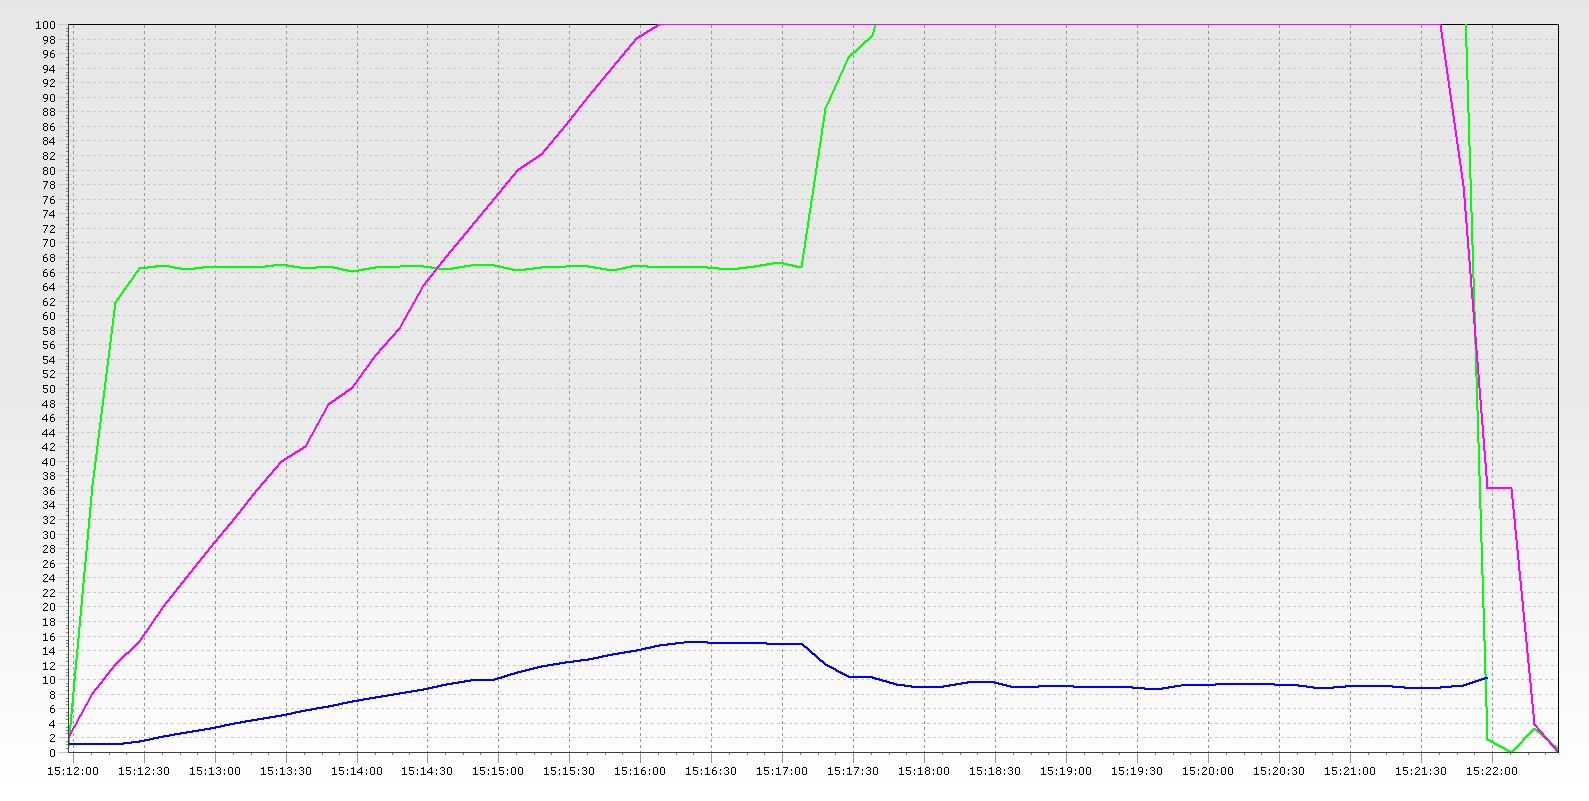
\includegraphics[width=1\textwidth]{../pic/Cluster-Async-Test-Overview.jpg}
\label{fig:test}
\end{figure}

%\clearpage

\section{Fazit}

AKKA ist ein mächtiges Framework, mit welchem man sehr gut und einfach reaktive Anwendungen bauen kann. Jedoch muss man sich auch mit einem anderen Programmierparadigmer vertraut machen, welches am Anfang einige Tücken aufweist, wenn man die klassische synchrone Programmierung gewohnt ist. \\
\\
Ich sehe aber trotzdem einen großen Vorteil in diesem Framework, da man ohne bzw. mit kleinen Änderungen eine vertikal skalierbare Anwendung bekommt. Das ist eine der Eigenschaften, von der ich glaube, dass diese in Zukunft noch wichtiger wird, um die Resourcen (CPU, RAM) von Servern besser ausnutzen zu können. Besonders im Bereich von Cloud-Computing, wo man dynamisch Rechenleistung zu einer Anwendung hinzufügen und entfernen kann, ist der Ansatz aus diesem Projekt sehr interessant. Ich könnte mir gut vorstellen, dass man noch Analyser Aktoren zu solch einer Anwendung hinzufügen könnten, welche feststellen können, ob der Cluster überladen ist. Wenn das der Fall ist, könnte der Aktor automatisch eine weitere Cloud-Recheneinheit starten und zum Cluster hinzufügen. Damit könnte man super das 'Pay per Use' Konzept anwenden.\\
\\
Mir hat auch die Kombination aus Tomcat und AKKA in diesem Projekt sehr gut gefallen. Ich war verwundert, wie harmonisch man die beiden Frameworks miteinander verbinden kann.\\
\\
Der gesamte Code ist auch auf Github verfügbar\\ \href{https://github.com/thomasfischl/akka-sample-cluster}{https://github.com/thomasfischl/akka-sample-cluster}.

\end{document}
